%%%%%%%%%%%%%%%%%%%%%%%%%%%%%%%%%%%%%%%%%%%%%%%%%%%%%%%%%%%%%
%															%
% %CS_383_Assignment1_LaTeX_UML_Document					%
% LaTeX Template											%
% Version 1.0 (2/9/17)										%
%															%
%															%
% author: Adrian Beehner									%
%															%
%															%
% description: LaTeX document that contains memo and		%
%	appendicies for UML diagramming tools					%
%															%
%%%%%%%%%%%%%%%%%%%%%%%%%%%%%%%%%%%%%%%%%%%%%%%%%%%%%%%%%%%%%


% Set Up Document
\documentclass[12pt]{article}
\usepackage{titlesec} 
\usepackage{hyperref}
\usepackage{graphicx}
\usepackage{float}
\usepackage{parskip} % Adds spacing between paragraphs
\usepackage{xcolor} % For setting colors
\usepackage{listings}
\setlength{\parindent}{15pt} % Indent paragraphs
\usepackage[margin=1in]{geometry}

% Make so Picture/floats go at top of page
\makeatletter
\setlength{\@fptop}{0pt}
\makeatother

% set the default code style
\lstset
{
	frame=tb, % draw a frame at the top and bottom of the code block
	tabsize=3, % tab space width
	showstringspaces=false, % don't mark spaces in strings
	numbers=left, % display line numbers on the left
	commentstyle=\color{green}, % comment color
	keywordstyle=\color{blue}, % keyword color
	stringstyle=\color{red} % string color
}

% Make sure hyperlinks for table of contents and website links dont have wierd red box
\hypersetup{
	colorlinks,
	citecolor=black,
	filecolor=black,
	linkcolor=black,
	urlcolor=black
}

\begin{document}
	
	% Set up Manual Indenting
	\setlength{\parindent}{15pt}
	\newcommand{\forceindent}{\leavevmode{\parindent=2em\indent}}
	
	
	%----------------------------------------------------------------------------------------
	%	TABLE OF CONTENTS
	%----------------------------------------------------------------------------------------	
	% Create title Page
	\title{Updating Design Specification for Second Sprint Report}
	\author{Team 3 (Java)}
	\date{}
	\maketitle
	
	% Create Table of Contents
	\tableofcontents
	%Set Table of Content depth
	\setcounter{tocdepth}{3}		% Include \subsubsection in ToC
	% Create new Page
	\newpage
	
	%----------------------------------------------------------------------------------------
	%	APPENDICIES
	%----------------------------------------------------------------------------------------
	%Apendix Section
	\appendix
	
		%----------------------------------------------------------------------------------------
		%	APPENDIX A Content - Sample Code/Work Done
		%----------------------------------------------------------------------------------------
		\section{Changes/Updates}
		\forceindent The changes made to the Design Specification was relatively small. These changes are listed below.
		
			%----------------------------------------------------------------------------------------
			%	Frame Preview Bar
			%----------------------------------------------------------------------------------------
			\subsection {Updating the Diagram for Grid Editor}
			\forceindent The change made to the diagram for the Grid Editor was to reconfigure the diagrams to accurately represent the current build of the system for the second sprint. The Color Class was removed from the diagram as the team opted to utilize Java's own built in Color Class. Two new classes were added in the diagram, a FrameButtonActionListener class, which does as it is named, and utilized to handle actions made to the "Frame Button" in the GUI. The other class was the NodeActionListner, which also performs as it is described, handling the button press of a node in the GUI. These diagrams thus were updated and reflected in the updated Design Specification for Sprint 2.
			
			%----------------------------------------------------------------------------------------
			%	Frame Preview Bar
			%----------------------------------------------------------------------------------------
			\subsection {Updating the Timeline}
			\forceindent The timeline was edited to reflect the progress the team has currently made since Sprint 2 and also display the goals the team hopes to accomplish in the following sprints. Originally, we had not exactly planned for a frame editor (which include the frame preview bar), but that is now reflected in the timeline, but since it is not done, it was moved to be completed at a later sprint. The Mulit Node Editor is the next goal as well, since the Single Node Editor is fully functioning now, as well as most  of the GUI elements. The timeline reflects the idea that due to the success of the team's progress, there will be additional time to add or edit features, however this is not set in stone as difficulties in the future may arise.
			
			% Create new Page
			\newpage
		
		%----------------------------------------------------------------------------------------
		%	APPENDIX B Content - Sample Code/Work Done
		%----------------------------------------------------------------------------------------
		\section{Added Section(s)}
		\forceindent Only one section was required to be added to Sprint 2, which was the TAN file section. These section(s) are further discussed below.
		
		%----------------------------------------------------------------------------------------
		%	Frame Preview Bar
		%----------------------------------------------------------------------------------------
		\subsection {TAN File Section}
		\forceindent The TAN file section was only just implemented into the Design Specification under Design Decisions due to the team not having the full picture of the requirements of the TAN file until the end of the last sprint. The TAN file section briefly explains the purpose of the TAN file, as well as providing a brief description of the components that make up the the TAN file. These components are then explained to be utilized so that the editor can read in files, and correctly output them to the GUI, as well as having the editor write out to files, allowing users to save these TAN files. The section was fairly extensive at explaining the properties of the TAN file and its functionality within the scope of the project.
		
		% Create new Page
		\newpage
		
		%----------------------------------------------------------------------------------------
		%	APPENDIX C Content - Diagrams for First Development Sprint
		%----------------------------------------------------------------------------------------
		\section{New/Changed Diagrams for Update}
		\forceindent The Following are diagrams were created/updated for relevancy in the updating the Design Specification for the second sprint, these diagrams are presented in the following sections below.
	
			%----------------------------------------------------------------------------------------
			%	CLASS DIAGRAM FOR COLOR, NODE, AND FRAME CLASS
			%----------------------------------------------------------------------------------------
			\subsection {Class Diagram for Grid Editor}
				\forceindent The Class Diagram below in Figure displays the structure of the Grid Editor (so far), in which the Color, Node, and ActionListener classes holds the main mechanism of the Gird Editor, also showing the relationships between these classes. This has been updated from the previous sprint, by removing the Color class (utilizing Java's default Color class) and adding the NodeActionListener class and FrameButtonActionListener class. The diagram is shown in Figure 1 below.
				
				\begin{figure}[ht!]
					\centering
					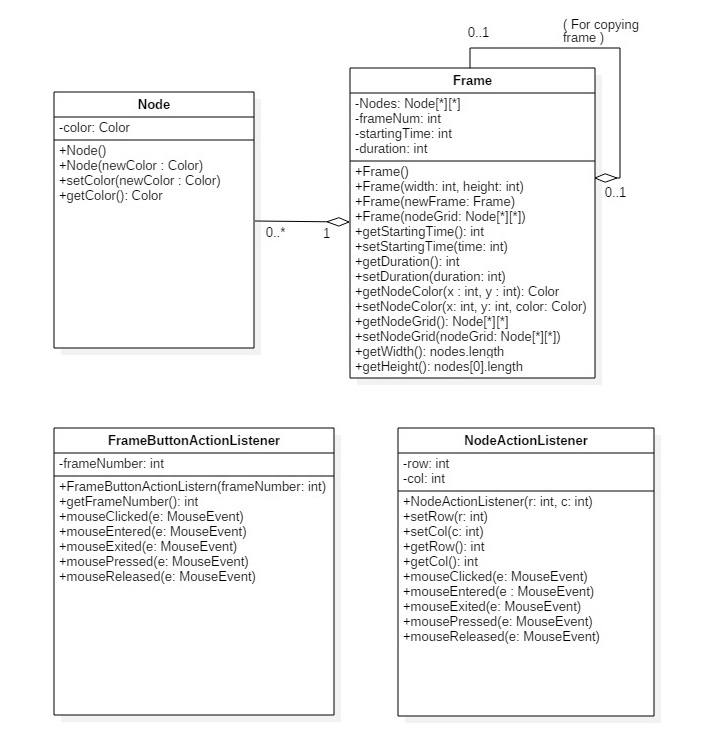
\includegraphics[width=120mm]{Class_Diagram_Frame_Node_and_ActionListener_Classes.JPG}
					\caption{Class Diagram of Grid Editor \label{overflow}}
				\end{figure}
			
			%----------------------------------------------------------------------------------------
			%	CLASS DIAGRAM FOR COLOR, NODE, AND FRAME CLASS
			%----------------------------------------------------------------------------------------
			\subsection {Frame Preview Bar Diagram}
			\forceindent The diagram in the figure below displays the structure of the Frame Preview Bar, which contains a list of frames, which have images to show the frame's configuration. There also exists a scroll bar as shown, which allows the user to scroll to show other frames. This diagram was mainly added to present the user with a visual cue to how the Frame Preview Bar should function. The diagram is shown in Figure 2 below.
			
			\begin{figure}[ht!]
				\centering
				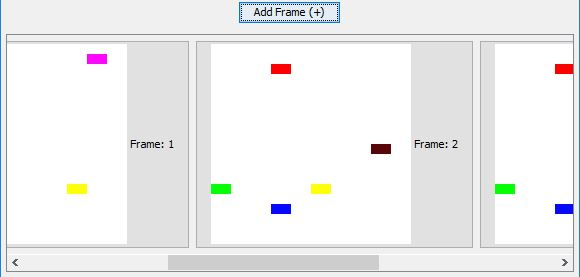
\includegraphics[width=120mm]{potoFramePre.JPG}
				\caption{Diagram of Frame Preview Bar \label{overflow}}
			\end{figure}
			
			%----------------------------------------------------------------------------------------
			%	CLASS DIAGRAM FOR COLOR, NODE, AND FRAME CLASS
			%----------------------------------------------------------------------------------------
			\subsection {Grid Editor Diagram}
			\forceindent The diagram in the figure below displays the structure of the Grid Editor in regards to the second sprint. This was shown to display the progress made on the Grid Editor GUI since the first sprint. The Grid Editor now displays a color when the user enter the RGB values of that color in the node dialog box. This effect was supposed to be focal point of the diagram. The diagram in shown in Figure 3 below.
			
			\begin{figure}[ht!]
				\centering
				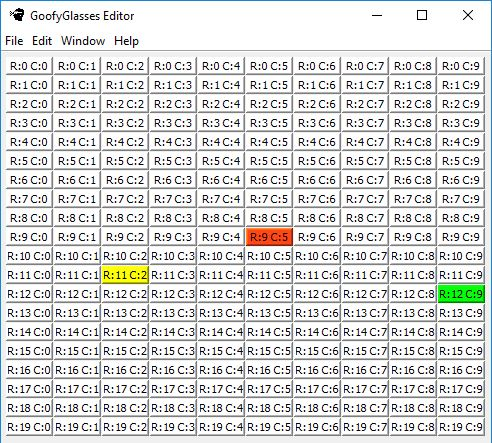
\includegraphics[width=120mm]{protoGrid.JPG}
				\caption{Diagram of Grid Editor \label{overflow}}
			\end{figure}
		
			
		
		% Create new Page (NEED TO USE clearpage because we have pictures that will affect it!)
		\clearpage
		
		
\end{document}